\chapter{Financialization} \label{chapter-financialization}
\epigraph{Financialization  occurs when housing is treated as a commodity—a vehicle for wealth and investment—rather than a social good.}{Special UN Rapporteur on the right to adequate housing, Leilani Farha}
%https://www.ohchr.org/en/special-procedures/sr-housing/financialization-housing
\epigraph{Financialization is a process whereby financial markets, financial institutions, and financial elites gain greater influence over economic policy and economic outcomes. Financialization transforms the functioning of economic systems at both the macro and micro levels.}{Thomas I. Palley \cite{palleyFinancializationWhatIt2007}}
%*** ADD MORE ON THE LITERATURE ON FINANCIALIZATION TO SETUP OUR WORK, AS IN THE ABOVE CHAPTERS
In this thesis we are focused on modelling the  effects of financialization on the urban housing market.  The term financialization is used in a variety of ways across a fairly wide range of contexts. In finance, it is  a term for the process of developing the legal instruments that facilitate financial transaction.  At the microeconomic level it is  a  collective noun for the growth in the number of individual transactions that create or transfer financial assets. At a macro level it refers to the effect on the system itself of the new instruments and the increase in the type of transaction that they make possible. It is the macro effects that are our main interest, but to model those in an \gls{ABM} we are forced to carefully specify the microeconomics of  individual decisions. 

We therefore begin in Section~\ref{section-financialize}  with a definition of the act of financializing transactions and markets,  and discuss some significant examples. In Section~\ref{section-micro} we describe the microeconomic objective function that individuals and our bank agent employ in deciding to purchase a property. Finally, in  
In Section~\ref{section-system} we explain how the term is applied at the level of systems and while markets and how finacialization might affect  the housing market as a system. At that point we can introduce our specific hypotheses and how we intend to test them.
% We therefore begin with a narrow and strict definition of the act of finacializing, followed by  an explanation and examples. We then go on to explain how the term is applied at the level of systems and while markets.

% At that point we can introduce our specific hypotheses and how we intend to test them.

\section{Financial instruments and financialization} \label{section-financialize}
The word ``financialization'' has several quite different meanings.  

%*YOU SAY ABOVE YOU ARE GOING TO NARROW TO A SPECIFC DEFINITION, CAN YOU MAKE VERY CLEAR HERE WHAT THAT IS. LIKE THESE ARE ALL POSSIBLE DEFINITIONS. THEN STATE VERY EXPLICITLY, THIS IS THE ONE WE ARE USING. 

To financialize anything is to create a  \gls{financial instrument} that represents it and can be bought and sold as an investment. Not all financial instruments are instruments of financialization. For example, mortgages are  financial instruments, but another step is required to create a financialized  market in mortgages. 

%*E i'M A BIT CONFUSED HERE... i THINK YOU ARE GOING INTO EXPLAINING HOW THEY BECAME FINANCIALIZED, BUT IT'S SET UP LIKE AND EXAMPLE... CAN YOU SAY WHERE YOU ARE GOING BEFORE OPENING THE DETAILS ABOUT THE MORTGAGE. lIKE THEY BECAME FINACICLAIZED OVER TIME... AT A BASI LEVEL A MORTGAGE MAKES POSSIBLE ETC..


\subsection{Mortgages}

Mortgages, for example, are a financial instrument that allows lenders to  participate in housing purchases in the present in exchange for a future flow of payments.  The mortgage does not create housing, but it enables the prospective buyer to become the nominal owner of an asset that produces a stream of benefits. The stream of benefits from secure housing near a source of income generally exceeds a buyer's current assets. The mortgage enables the  transfer of ownership because it makes it possible to transfer the rights to a substantial fraction of the future income of the buyer to the mortgage holder who, in effect, is the owner until the terms of the mortgage are fulfilled.  If the mortgagee fails to make those payments the mortgage holder repossess the asset. The security provided by this instrument ``de-risks'' the transaction, making it safer and therefore easier to achieve the mutual benefits of the sale.

Originally mortgages were an arrangement between just the buyer and the seller, but in the 1870s in the USA, insurance companies stepped into these transactions, paying off the seller and then collecting the principle and interest payments on behalf of the bank's shareholders. This innovation was an example of financialization that made it possible for individual insurance companies to profit by providing money to buyers. When mortgage lending was regulated and insured  by the American government during and after the great depression it facilitated a massive increase in home ownership in the USA and contributed to the post-war construction boom and the suburbanization of American cities. 

These mortgages were still agreements between individual lenders and buyers. When financial institutions developed markets that let them buy and sell bundles of mortgages among themselves, we say the mortgage market itself was financialized. There was then a market for the  promises to pay in addition to the underlying market for housing and the market for mortgage-type loans loans

The transactions in this market do not directly affect the mortgage conditions or the home: they simply add a new product for investors or banks to buy and sell. This new market was thought to further reduce the risk for lenders, but  between 2007 and 2010 in the USA the sub-prime mortgage crisis destabilized the financial institutions that were playing this new market. \footnote{As I understand it, that crisis resulted from overselling risky and predatory mortgages by lenders with more money to lend than the market could absorb. Eager investors seeking higher or more secure returns were willing  to buy bundles of  mortgages that were in theory de-risked. Pooling uncorrelated individual risk, as the insurance industry does, produces lower overall risk. (The instruments that enabled the speculative bubble were mortgage-backed securities (MBSes) and collateralized debt obligations (CDOs).) Pooling does not reduce systemic risk, however. As it turned out, the mortgage default rate rose, lenders' liquidity fell, mortgage rates were pushed up, defaults increased, and the market for the new instruments collapsed, taking down major financial institutions. The details don't matter for this thesis, but they provide a cautionary tale about the the potential costs of financialization.}.  

About 80\% of Canadian homes are owner-occupied and about a third of the value of the homes is held as mortgages. Approximately two-thirds of the net land rents associated with housing, therefore, accrue to owner-occupiers \cite{nemtinFinancializationHousingSocial2021}. {\color {red}CHECK THESE NUMBERS AND IF THEY CITE A BETTER SOURCE WE SHOULD GET} 

The mortgage demonstrates the two aspects of financial instruments. It is both a financial instrument that enables  purchase and a financial asset that can be bought and sold. When we consider urban housing, it is the right to future income generated by capital, labour, and the city itself through the agglomeration effects that drive productivity. It is an instrument that indirectly captures a share of the urban rents. As productivity rises, wages rise, rents rise, property prices rise and mortgages rise. 

For urban theory and policy formation it is important to distinguish between financial instruments that enable production of real assets, and instruments like  mortgages that primarily facilitate the transfer of real assets or rights to real estate  income. Housing developers borrow to purchase land for development and builders borrow to finance construction. While important, the financial instruments involved are not driving the financialization of housing.  The size of the loans involved is affected by the amount of land purchased and the potential rents earned by that land, but the degree of non-occupant ownership is not affected. *** CLARIFY

  \begin{figure}
\begin{center}
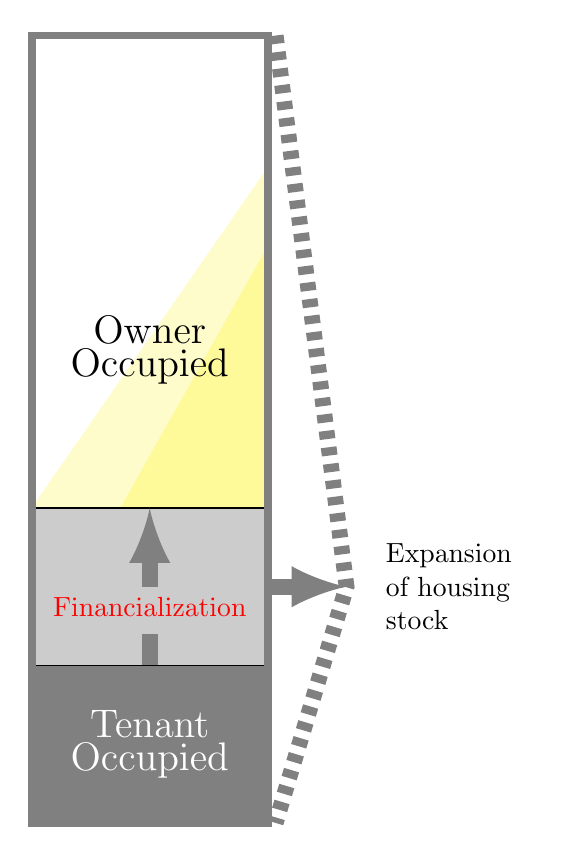
\begin{tikzpicture}{scale=.5}
\draw [fill=yellow!20] (0,4)--(3,4)--(3,8.33); --cycle;% MORTGAGE %Calculation. 80\%owner, so  8 above the tenant line. 2/3*8=5.333. 5.333+2=

\draw [fill=yellow!40] (0,2)--(3,2)--(3,7.33); --cycle;% MORTGAGE %Calculation. 80\%owner, so  8 above the tenant line. 2/3*8=5.333. 5.333+2=
 \draw [fill=gray!40,opacity=1] (0,0) rectangle (3,4); %fiancialization   
\draw [fill=gray] (0,0) rectangle (3,2); %TENANT

\draw[line width= 1mm, black!50] (0,0) rectangle (3,10);

\node at (1.5,6)
    [text width=2.4cm, align=center]
    {\baselineskip=20pt\Large Owner Occupied};
%\node at (2,3.3) [text width=2.4cm]  {\baselineskip=20pt Mortgaged};
\node at (1.5,1)
    [text width=2.4cm, align=center, white]
    {\baselineskip=20pt\Large Tenant Occupied};


%\draw [gray,line width=2mm](1.5,2)--(1.5,2.4) node[above, red]{Financialization}; 
\draw [gray,line width=2mm](1.5,2)--(1.5,2.4) node[above, red]{Financialization}; 
\draw [gray,-latex, line width=2mm](1.5,3)--(1.5,4);
\draw [gray,line width=2mm,-latex](3,3)--(4,3); \node at (5.5,3)[text width=2cm]{Expansion of housing stock}; 
\draw [gray, dashed,line width=2mm,](3.1,10)--(4,3)--(3.1,0);
\end{tikzpicture}
\end{center}
 \caption{Financialization vs expansion of the housing stock }
      \label{fig:Financialization-expansion}
  \end{figure}

%*E IF YOU SAY IT WAS THOUGHT TO LOWER RISK, CAN YOU FINISH THAT THOUGHT. %DID THE CRISIS SHOW IT DIDN'T? OR IS IT UNCLEAR WHETHER IT DOES? iS IT A DEBATED POINT? OR CHEANGE THE SENTENCE SO YOU DON'T SET UP IT WAS THOUGHT AND LEAVE THE CONCLUSION HANGING...

\subsection{Stocks and stock markets}
The \gls{joint stock company}, the basis of the modern stock market and an important mechanism for channeling investment  into productive activity,  is probably the most important financial instrument in the capitalist economy. Originally a tool to allow a group of investors to pool their money, take on large projects, and to share risks, the stocks themselves rapidly became objects of trade and speculation. Share prices on the stock market are not tightly tied to the productivity of the company they represent, which makes it clear that the financial instrument is something different from the real asset. 

Stock markets are  generally described as a primary means of efficiently mobilizing long term savings and investment for  fixed capital formation.\cite{azfarMarketMobilizedCapital2003} Most stock transactions however are speculative in nature and there is significant disagreement about the link between stock investment and investment in productive real assets.\footnote{Mork et. al \cite{morckStockMarketInvestment1990} identify four theories that attempt to explain the correlation between stock returns and subsequent investment \begin{quotation}The first says that the stock market is a passive predictor of future activity that managers do not rely on to make investment decisions. The second theory says that, in making investment decisions, managers rely on the stock market as a source of information, which may or may not be correct about future fundamentals. The third theory, which is perhaps the most common view of the stock markets influence, says that the stock market affects investment through its influence on the cost of funds and external financing. Finally, the fourth theory says that the stock market exerts pressure on investment quite aside from its informational and financing role, because managers have to cater to investors' opinions in order to protect their livelihood. For example, a low stock price may increase the probability of a takeover or a forced removal of top management.If the market is pessimistic about the firm's profitability, top management may be deterred from investing heavily by the prospect of further erosion in the stock  price.\end{quotation} None of the point to a direct connection between stock market investment and real investment.}  Mutual funds, which pool risky stocks, are a derivative  financial instrument built on top of the stock market.


\subsection{Investment trusts}
An example of a financial instrument designed specifically to support rent extraction and which  increases the degree of financialization of the housing supply is the  Real Estate Investment Trust (REIT).  A REIT is a company that owns, operates, or finances income-generating real estate and distribute the income to shareholders. While the company itself is an management system, the shares are are simply financial assets that are that are sold to individuals and organizations that want to share in real estate revenues and capital gains. There are other large owners of residential real estate such as life insurance companies and pension plans that behave similarly, but REITs are a relatively new financial instrument which is  expanding rapidly and attracting political attention for their effect on housing markets.  % REITs that develop new properties generally don't sell the properties they construct.

REITs have become increasingly popular in recent years.  An S\&P-Dow Jones research bulletin reported that over the  25 years to 2017, REITs outperformed stocks, bonds, and commodities \cite{GET-Dow-Jones-research-bulletin}. Because they have outperformed competing investments they have attracted  capital from other uses.

Developed in the USA  in 1960 (as an amendment to the Cigar Excise Tax Extension!) and in Canada in 1993 \cite{GET_REITsDevelopedDates}, REITs are similar to mutual funds in making it possible for an individual, often small investors to earn dividends from real estate investments without having to buy, manage, or finance any properties themselves. There are questions about preferential tax treatment, and whether some REITs are really just inappropriately sheltered real-estate corporations.  For the purpose of this thesis, they are simply one of the mechanisms for the financialization of housing.

They are not simply a neutral tool for saving however. According to a paper \cite{wangAnalyzeImpactREITs2021} on REITS in the Irish housing market, ``REIT successfully reconnected the international financial market and the Irish real estate market.'' In other words, in Ireland, REITS have made it easier for international capital to buy Irish land. The entry of outside and footloose capital has had an effect on the resident population:  ``the large-scale acquisition of Irish real estate by REITs and other real estate buyers has also caused some new problems. First, the active management of assets by REITs and other investors has led to a rapid increase in rents''.\footnote{In  IMF working paper ``Capital Account Liberalization and Inequality'' \cite{furceriCapitalAccountLiberalization2015}  Furceri and Loungani reported that that for 149 countries from 1970 to 2010, ``after countries take steps to open their capital account, an increase in inequality in incomes within countries follows'' . The observation is consistent with our argument  that domestic rent-seeking in housing markets will increase inequality.}   

There is evidence that REITs affect real estate markets in other ways. Bat et all  \cite{batRolePublicREITs2022} reprot that  ``they are actually financial actors that aggressively buy up property assets and manage them to extract wealth at taxpayers’ expense. '' and ``they have expanded the pool of capital available for transactions that monetize real property and turn it into tradable assets – financial widgets with little or no connection to the real purpose of the productive enterprises that occupy the properties they own.''





\subsection{Financial instruments and financialization: a final comment}
We have called attention in this section to the development  several important financial instruments -- mortgages, stocks, and REITs --  with the intention of  disentangling the concept of financial instruments from the term ``financialization''.  We say that financialization is occurring if there is an  increase the stock of financial assets associated with a stock of real assets. The development of new instruments facilitates this process. 

\section{The microeconomics of  financialization}\label{section-micro}

At  the microeconomic level, where individual decisions are made, financialization happens,  real assets are bought by individuals and institutions. Individual home-buyers are buying a stream of housing services and possible capital gains. Institutional buyers are buying a stream of net rents plus speculative gains. Each agent has their own interest rates, discount rates, mortgage share, information, and expectations, so individual bids can differ.



%In the process, the real asset takes on an additional and separate aspect as financial object that can be bought and sold. 

The feature that matters most to investors is the  \gls{rate of return} that  an asset offers. For any level of risk and liquidity, an investor will choose to purchase the asset with the highest rate of return. When a home is bought to live in, the potential buyer makes a similar calculation, perhaps with a greater emphasis on the value of the stream of housing services. When home prices are rising rapidly speculative gains may become the dominant concern of home buyers. 

To model the investment decision  we therefore need to calculate the \gls{rate of return} on each property taking into account the rental revenue, the potential capital gain, the investors' costs of capital, incomes, and assets. The analysis will show the incentive structure driving the  financialization of the housing market. We do this in detail in Appendix~\ref{appendix-bid-price} 


We first calculate the net present value of the purchase, then divide by the amount of capital employed, which we assume is simply the size of the down payment made at the beginning of the period. This gives us a rate of return.\footnote{A common approach would be to calculate an internal rate of return (IRR), but  the IRR is in general the solution to a polynomial and does not guarantee a single-valued result.\cite{robinsonOPTIMALTERMINATIONIRR1996} Multiple real-valued  IRRs may arise;  complex-valued IRRs may arise;  the IRR is, in general, incompatible with the net present value (NPV) in accept/reject decisions; the IRR ranking is, in general, different from the NPV ranking; the IRR criterion is not applicable with variable costs of capital. Ways to salvage the IRR as a usable criterion have been proposed that are consistent with our approach \cite{magniAverageInternalRate2010}, which is to calculate an NPV then convert it to a rate,} 

\begin{eqnarray}
Rate\ of\ return\ on\ capital\ invested = \frac{\delta \left((1+ \dot P_M^e - (1+r)m\right)}{1-m} + \frac{\mathcal{R}_N}{(1-m)P_B}\label{equation-RoR}
\end{eqnarray}
where 

\begin{tabular}{lll}
 $\delta$       &=& individual discount rate \\
$\dot P_M^e $   &=& expected rate of price increase \\
$ r$            &=& mortgage interest rate \\
$m$             &=&  fraction of the price that can be mortgaged \\,
$ \mathcal{R}_N$ &=&  net rent
\end{tabular}
Equation~\ref{equation-RoR} makes it clear that the estimated rate of return depends on subjective magnitudes,$\delta$ and $\dot P_M^e$, attributes of the property, $ \mathcal{R}_N$, and  individual financial position, $r$, $m$.

The individual's Rate of return on capital  invested  for each project  is compared to the investor's target rate, $r_{target}$, providing  an investment criterion:
\begin{eqnarray}
r_{target} \le \frac{\delta \left((1+ \dot P_M^e - (1+r)m\right)}{1-m} + \frac{\mathcal{R}_N}{(1-m)P_B}
\end{eqnarray}
In Appendix~\ref{appendix-bid-price} this expression is solved for $P_B$, the  maximum price that allows the investor can pay and still achieve at least her  target rate of return, $r_{target}$.  

\begin{eqnarray}
P_B & \le    \frac{\mathcal{R}_N}{(1-m)r^{target}-\delta \left(1 + \dot P_M^e - (1+r)m\right)} \label{equation-Bidprice}\end{eqnarray}
% P_B & \le    \frac{\mathcal{R}_N}{(1-m)r^{target}-\left[ \delta(1+L(P)- (1+r)m\right]}
We call this  $i's$ maximum bid and compute it for all potential buyers. In each sale the highest $P_B$ will make the purchase. The denominator can be seen as an adjusted rate of return for capitalizing net rents, analogous to the value of $r$ in  the standard capitalization formula.


The market mechanism then simply has to compare the bid price  $P_B$ with the seller's reservation price and apply a bargaining rule to determine how any surplus is allocated.


 Since  agents do not have perfect information, the calculation is done with their best approximation of values. % The agent does not know the future. 
 The rate of price growth $\dot P$, is an approximation based on rents and past market behaviour.\footnote{Case and Shiller ``..we see a market largely driven by expectations. People seem to form their expectations from past price movements rather than having any knowledge of fundamentals. This means that housing price booms will persist as home buyers become destabilizing speculators.''Case and Schiller, \cite{caseThereBubbleHousing2003}} Details of the derivations, and implementation, are discussed in the Appendix. % We calculate the bid price in Appendix \ref{appendix-bid-price}.

 
%Thus, the 1-year expectations are fairly well described as attenuated versions of lagged actual 1-year price changes, Case and Schiller, \cite{caseThereBubbleHousing2003} p282

%  GET?? Case, Karl E., and Robert J. Shiller. 1988. “The Behavior of Home Buyers in Boom and Postboom Markets.” New England Economic Review (November– December), pp. 29–46.



\subsection{Implications of the bidding rule}

\begin{enumerate}
\item A large $m$ magnifies the return. (The downpayment is smaller as a fraction of the price, increasing the investor's leverage). 
Given the  common rule that mortgage payments cannot exceed some fraction of disposable income, the wealthy will be able to borrow larger amounts and at lower interest rates than the less wealthy. At any distance from the centre they will be able to make a higher bid.

\item A lower mortgage interest rate increases the return by lowering interest payments. The cost of capital is known to differ for rich and poor.  The wealthy can generally borrow  at lower interest rates than the less wealthy. 

\item A lower discount rate $\delta$ reduces the subjective rate of return.  Poverty in assets and cash liquidity constraints are correlated with higher rates of time preference  \cite{carvalhoPovertyTimePreference2010}\cite{holdenPovertyMarketImperfections1998}. If agents discount at their borrowing rate, wealthier agents may have a lower subjective rate of time preference and therefore value properties more highly. 

\item Higher expected price appreciation increases the attractiveness of an investment. Financial corporations and the wealthy are likely to have better price forecasts than  the occasional home buyer.
\item Higher rents make the unit more profitable. Higher expected  rents may result from expecting greater price appreciation  leading to raising rents for tenants. Lower discount rates may give future rent increases greater present value.
\item Lower maintenance costs increase profits. There may be scale economies in the maintenance  of rented housing. 
\item Lower tax rates decrease holding costs and increase the value of the investment. There may be opportunities to shelter income with land held for investment (speculative) purposes. Tax treatment of income and capital gains as well as interest deductibility may also provide advantyages for institutional buyers and investors.%\footnote{Case and Schiller \cite{LOST_CaseandSchiller} observe that (source?) `` ... increases in real per capita income all are positively related to excess returns or price changes over the subsequent year.''} 


\end{enumerate}
Some  of these conditions (1-3) hold generally for wealthier actors. Others (4-7) may be available only to institutional investors.  Financial corporations in particular may have advantages relative to individual investors, making it  reasonable to expect that financial corporations increasingly dominate urban land 
markets.\footnote{Fr\'ed\'erick Demers \cite{demersModellingForecastingHousing2005} found that the response of housing investment to interest rates has become more pronounced over time. This suggests a rising share of financial investors relative to buyers focused on housing services. Case and Schiller \cite{caseThereBubbleHousing2003} observe that  `` ... increases in real per capita income all are positively related to excess returns or price changes over the subsequent year.''}  

Since interest rates are lower for those with higher wealth, the analysis implies, consistent with the empirical evidence, that net returns for investment are increasing with wealth. Large wealth holders will get higher expected and actual rates of return on land than those with lower wealth holdings. Managers of large pools of capital will have an even greater   advantage.\footnote{ Equation~\ref{Eqn:DecisionRule} implies  sales go to the richest participant unless there are limits on the size of capital flows. For our simulation, we implement such limits. } 

 \footnote{Case and Schiller \cite{LOST_CaseandSchiller} observe that (source?) 
 `` ... increases in real per capita income all are positively related to excess returns or price changes over the subsequent year.''} 

The overall implication of Equation~\ref{equation-Bidprice} is that those with more capital will be at an advantage in the urban housing  market. 

 %The conclusion that we draw from the analysis above is that  financialization of urban housing benefits a rentier class of urban landholders. There is evidence that it benefits a globally distributed class of rentiers.  

\section{Financialization as system change}\label{section-system}

Financialization of the housing market is therefore the increasing control of the stock of urban land and housing in order to capture the scarcity rent generated by the people of the city.  Mortgages and REITs are both financial instruments.
*e tHIS IS CLEAR BUT COULD BE HELPED BY RESTATING HOW THEY MOVE IT ONTO FINANCIAL MARKETS. JUST A QUICK SUMMARY STATEMENT OF HOW THEY ARE FINACIALIZATION. %EVEN JUST something like... They put the ownership of housing onto financial markets. just to keep us oriented in what we are talkign about.

*E I FEEL LIKE THERE IS SOMETHING MISSING BETWEEN THESE TWO PARGRAPHS. %PERHAPS JUST FLESHING OUT WHAT FINANCIALIZATION LOOKS LIKE TECHNICALLY. MAYBE ALSO INSTRODUCE POSIBLE EFFECTS... LIKE EVEN JUST INTRODUCE THEM AS QUESTIONS? IT'S BEEN SUGGESTED OR SHOWN THAT ITS CONTRIBUTING TO THE HOUSING CRISIS. tHIS WOULD ALSO BE A GOOD PLACE TO EXAPLIN WHAT YOU MEAN BY "aS SYSTEMS CHANGE... BECAUSE i THINK THAT IS A BIG PART OF WHY YOU SAY NEXT THAT IT NEEDS TO BE UNDERSTOOD... BECAUSE IT HAS SUC BROAD EFFECTS

We need to understand the economics of financialization.
% \section{Literature on theory and evidence} % PROVIDE EVIDENCE 	mention theories?
There is substantial evidence that the financialization of urban housing is underway in Canadian cities..

Two questions arise when we observe the growing participation of global capital in the urban housing system: 
\begin{enumerate}
\item How far will the financialization of urban land go? 
\item That are the implications for the urban economy and the welfare of the urban population? 
\end{enumerate}

We can demonstrate that in the absence of policy interventions, differential access to finance capital ensures that capital owners acquire an increasing share of urban land % over time
and therefore capture the growing land rents from urban productivity growth. 

With this insight, growing wealth inequality emerges within a simple, widely accepted model of the urban land market. In the limit, urban residents are tenants, and new residents without capital no longer receive any of the increases in rents arising from the growing productivity of the city. 

%The first question, therefore, is reduced to which capital holders will increase their share of urban land and whether there is any reason to expect the process of financialization process to stop or reverse itself.

% \section{The incentives for financialization}
%Instead, drawing on the ideas of Jane Jacobs, Lucas proposes the city as the unit of analysis. Lucas, Robert (1990), "Why Doesn't Capital Flow from Rich to Poor Countries?," American Economic Review Papers and Proceedings v. 80, no. 2 (May) pp. 92-96.  
%Jacobs, Jane  (1969), The Economy of Cities (New York: Random House).  
% The Death and Life of Great American Cities \cite{jacobsDeathLifeGreat1961}


 MOVE The mortgage share and interest rate are functions of the agents wealth %Both the  share of the price  that can be mortgaged, $m$, and the interest rate and the interest rate paid, $r$, are functions of the agent's wealth. 
The discounting factor may be correlated with wealth as well. 

%%%%%%%%  VVVVVVVVVVVVVVVVVVVVVVV   This section May 18 to cut?  V
%%%%%%%%  ^^^^^^^^^^^^^^^^^^^^^^^   This section May 18 to cut?  V
% TODO - add interest rate discussion - (borrowing rates drive land prices up, even if there is no development or improvements, simply because it makes it worth a larger--the effect of low rates, especially for institutional actors have driven a large effect)
%\begin{enumerate}
%
%\item  the buyer and seller calculate the value of the property  differently. 
%
%\item  the  buyer and seller may have different expectations of the path of prices and therefore the stream of rents.
%%There are two standard ways that expectations are modeled
%%	\begin{enumerate}
%%	\item \textbf{Adaptive expectations.} Expectations are largely based on what has happened in the past. 
%%	Under normal conditions most people  have relatively weak incentive to get forecasts about inflation correct and lack the resources and time to purchase expert advice. 
%%	Recent price trends are easily available and likely to be the main source of  information.
%%	\item     \textbf{Rational expectations.} Expectations are based on a model of the future economy. 
%%International investors and banks employ economists and other experts to  forecast prices, exchange rates, and trends in the economy.
%%	\end{enumerate} 
%\end{enumerate}
% Why would  discount rates differ between identical workers? Buyers and sellers are not identical in wealth, . 
%%We could implement the first  explanation either by generating expectational errors based on functional class or wealth. 



\subsection{Financialization and productivity}

When  a productive asset is acquired as a financial asset it remains productive.  The financial instrument is separate form the real asset, at least in principle, and is traded in different markets. Why then is financialization an issue?  Theory suggests that financialization is positive.  The major argument is that finacialization enables real investment. In theory then, financialization of the housing market therefore  to more housing production. It is striking that after 40 years of growing financialization across we face a hosuing crisis , increasing homelessness and falling rates of homw ownership.  Palley \cite{palleyFinancializationWhatIt2007} reproits that 

\begin{quotation}At the macroeconomic level the era of financialization has been associated with generally tepid economic growth.\dots  In all countries except the U.K., average annual growth fell during the era of financialization that set in after 1979. Additionally, growth also appears to show a slowing trend so that growth in the 1980s was higher than in the 1990s, which in turn was higher than in the 2000s. \end{quotation}

%African land or land in Northern Ontario 
%Land acquired by holding companies may even be made more productive. The theory is that 
% the goal of such investments, however, is generally to achieve a capital gain over time. Financial analysis is essentially about rates of return on financial capital invested. The opportunity for capital gains  attracts financial capital to the housing market.%Financial managers have no interest is n in assets that are not expected to increase in value. 



*IT WOULD BE HELPFUL TO CONNECT FINANCIALZATION TO KEY THREAD FROM PAST CHAPTERS AT SOME POINT EVEN IF BRIEFLY